\documentclass[a4paper,12pt]{article}
% \usepackage[utf8]{inputenc}
\usepackage{parskip}
% \usepackage[sorting=none]{biblatex}
% \usepackage{url}
\usepackage{epsfig}
\usepackage{graphics}
\usepackage{fancyhdr}

\usepackage{mathtools}
% \usepackage{graphicx}
\usepackage[justification=centering]{caption}
\usepackage{caption}
\usepackage{subcaption}
\usepackage{amssymb}
\usepackage{amsmath}
\usepackage{tabularx}
\usepackage{xcolor}
\usepackage{multirow}
\usepackage{graphicx}
\usepackage{xcolor}
\usepackage{arydshln}
\usepackage{tikz}

\usetikzlibrary{shapes.geometric, arrows}


\newcommand*{\progName}[1]{\mbox{\texttt{#1}}}

\usepackage{geometry}
\geometry{
  paper=a4paper,
  margin=54pt,
  includeheadfoot
}

% \documentclass{amsart}

% \usepackage[margin=1in]{geometry}        
\usepackage[utf8]{inputenc} % allow utf-8 input
\usepackage[T1]{fontenc}    % use 8-bit T1 fonts
\usepackage{hyperref}       % hyperlinks
\usepackage{url}            % simple URL typesetting
\usepackage{booktabs}       % professional-quality tables
% \usepackage{amsfonts}       % blackboard math symbols
\usepackage{nicefrac}       % compact symbols for 1/2, etc.
\usepackage{microtype}      % microtypography
\usepackage{amsmath,amsfonts,amssymb}
% \usepackage{todonotes}

\usepackage{algorithm}
\usepackage{algpseudocode}

\usepackage[english]{babel}
\newtheorem{theorem}{Theorem}
\usepackage{soul}

\DeclareMathOperator*{\argmax}{arg\,max}
\DeclareMathOperator*{\argmin}{arg\,min}

%package for references
\usepackage[backend=biber, style=alphabetic, sorting=anyt]{biblatex}
\usepackage{csquotes}

\addbibresource{sources.bib}


\title{Pacman Capture the Flag \\ Assignment 4 Report}

\author{\hspace*{-0.5cm}
GROUP 03\\
\begin{tabular}{cccc}
Shekhar Devm Upadhyay & Aiman Shenawa\\
20010531 & 001021 \\
sdup@kth.se & ashenawa@kth.se \\
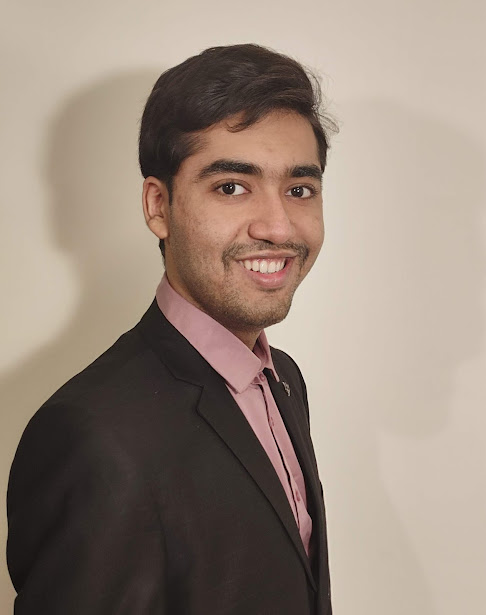
\includegraphics[width=0.2\linewidth]{side_profile.jpg} & 
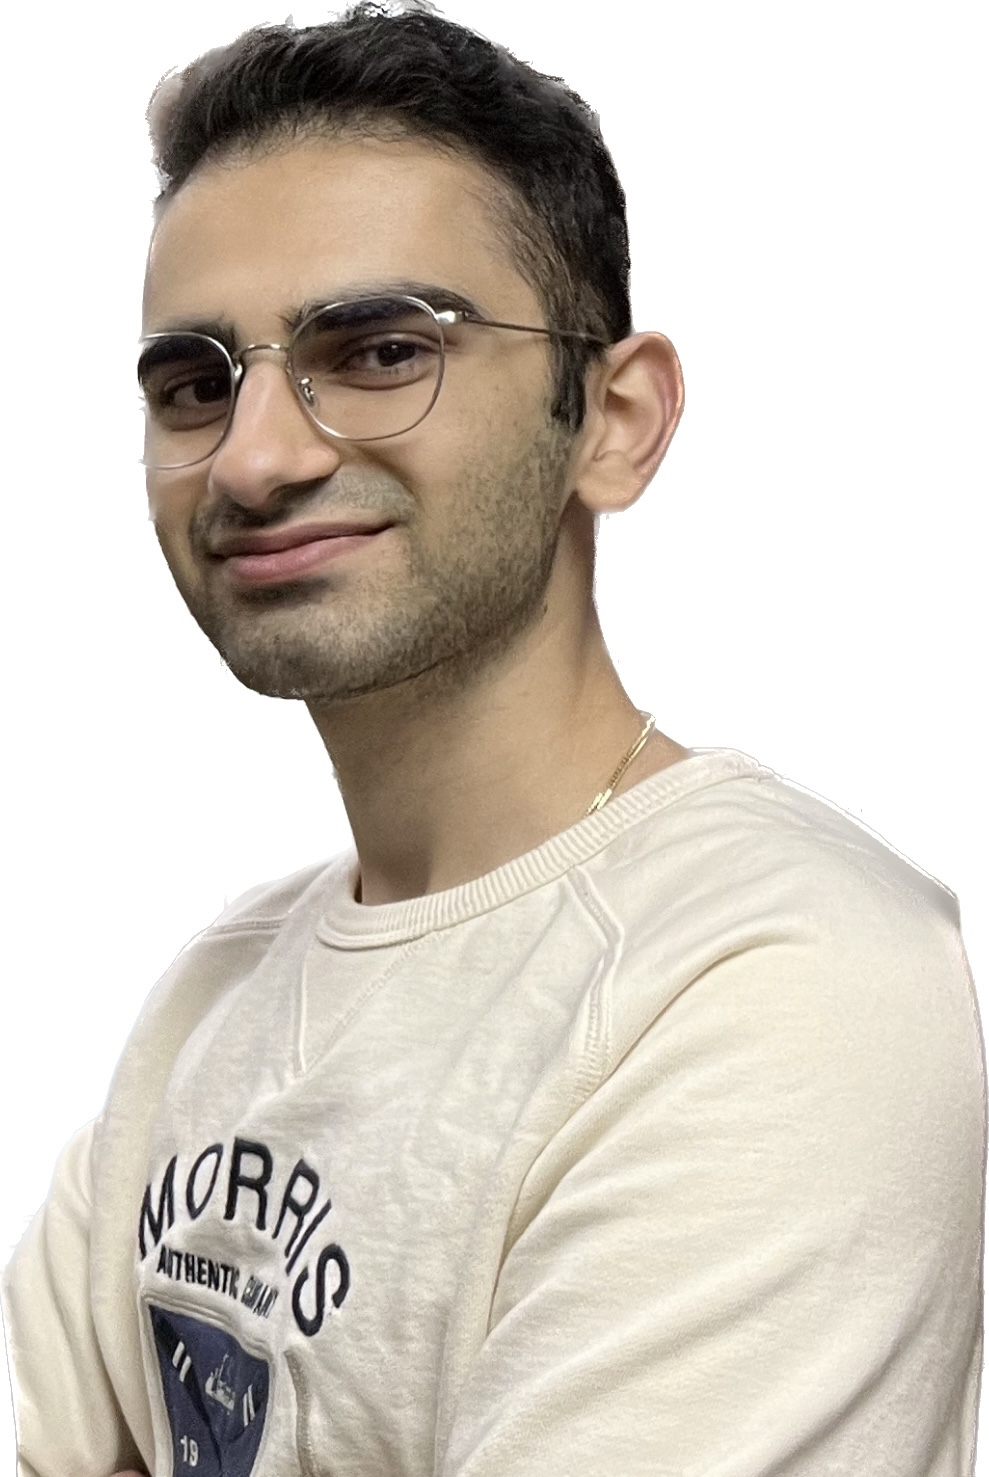
\includegraphics[width=0.17\linewidth]{Aiman_picture.jpg}
\end{tabular}} 
\date{May 2023}

% \pagestyle{fancy}
\setlength{\headheight}{15pt}
\fancyhf{}
\lhead{DD2438} % DO NOT REMOVE!!!!
\rhead{Shekhar Devm Upadhyay, Aiman Shenawa} %% UPDATE WITH YOUR NAMES

\addbibresource{sources.bib}

\begin{document}

\maketitle
\thispagestyle{fancy}

\begin{abstract}
% Describe the problem and importance in detail
% why it is important to study

% introduce pacman capture the flag problem
This report presents a study on the development of AI agents for controlling a team of two in a competitive Pac-Man Capture the Flag (CTF) scenario. The objective of the agents is to maximize their score by efficiently collecting food from the enemy turf within a limited number of moves. This report studies various approaches used in the field of artificial intelligence, including minimax game tree search, modifications like alpha-beta pruning and move ordering, Monte Carlo Tree Search (MCTS), Expectimax, and decision-tree-based approaches, presents the final solution employed by the authors, and does a comparative analysis of the approaches utilized by all the teams in the competition. By analyzing and comparing these strategies, we aim to identify effective techniques for AI-controlled agents in Pac-Man CTF.

\end{abstract}
\clearpage

%% REMEMBER TO WRITE IN A TOP-DOWN FASHION, STARTING EACH SECTION WITH A SUMMARY. 

\section{Introduction}
\label{sec:introduction}
% Describe the problem and importance in detail

With the continious development of society and technology, the need for autonomous agents is increasing. It is becoming more and more important to develop agents that can operate in dynamic and complex environments autonomously.
In this report we will explore the problem of developing an agent that can play the game of Pacman capture the flag. This is a project developed by UC Berkely, it is a challenge that combines classic video game mechanics with artificial intelligence techniques.
The goal of the project is to develop an agent that can play the game of Pacman capture the flag. The game is played on a grid, where the agent can move in four directions, up, down, left and right. 
The grid is split into two halves, in each half there is a team of Pacman agents, the goal of the game is to capture the food pellets from the other team's side and bring them back to your side while also preventing the other team from doing the same.
Multiple aspects of artificial intelligence will be explored in this report, such as minimax game tree search, Monte Carlo Tree Search (MCTS), Expectimax, and decision-tree-based approaches. The final solution included the use of Minimax and alpha-beta pruning.




% include new figure from folder figuresA4,
% figure showing the game environment
%insert figure
\begin{figure}[!htbp]
  \centering
  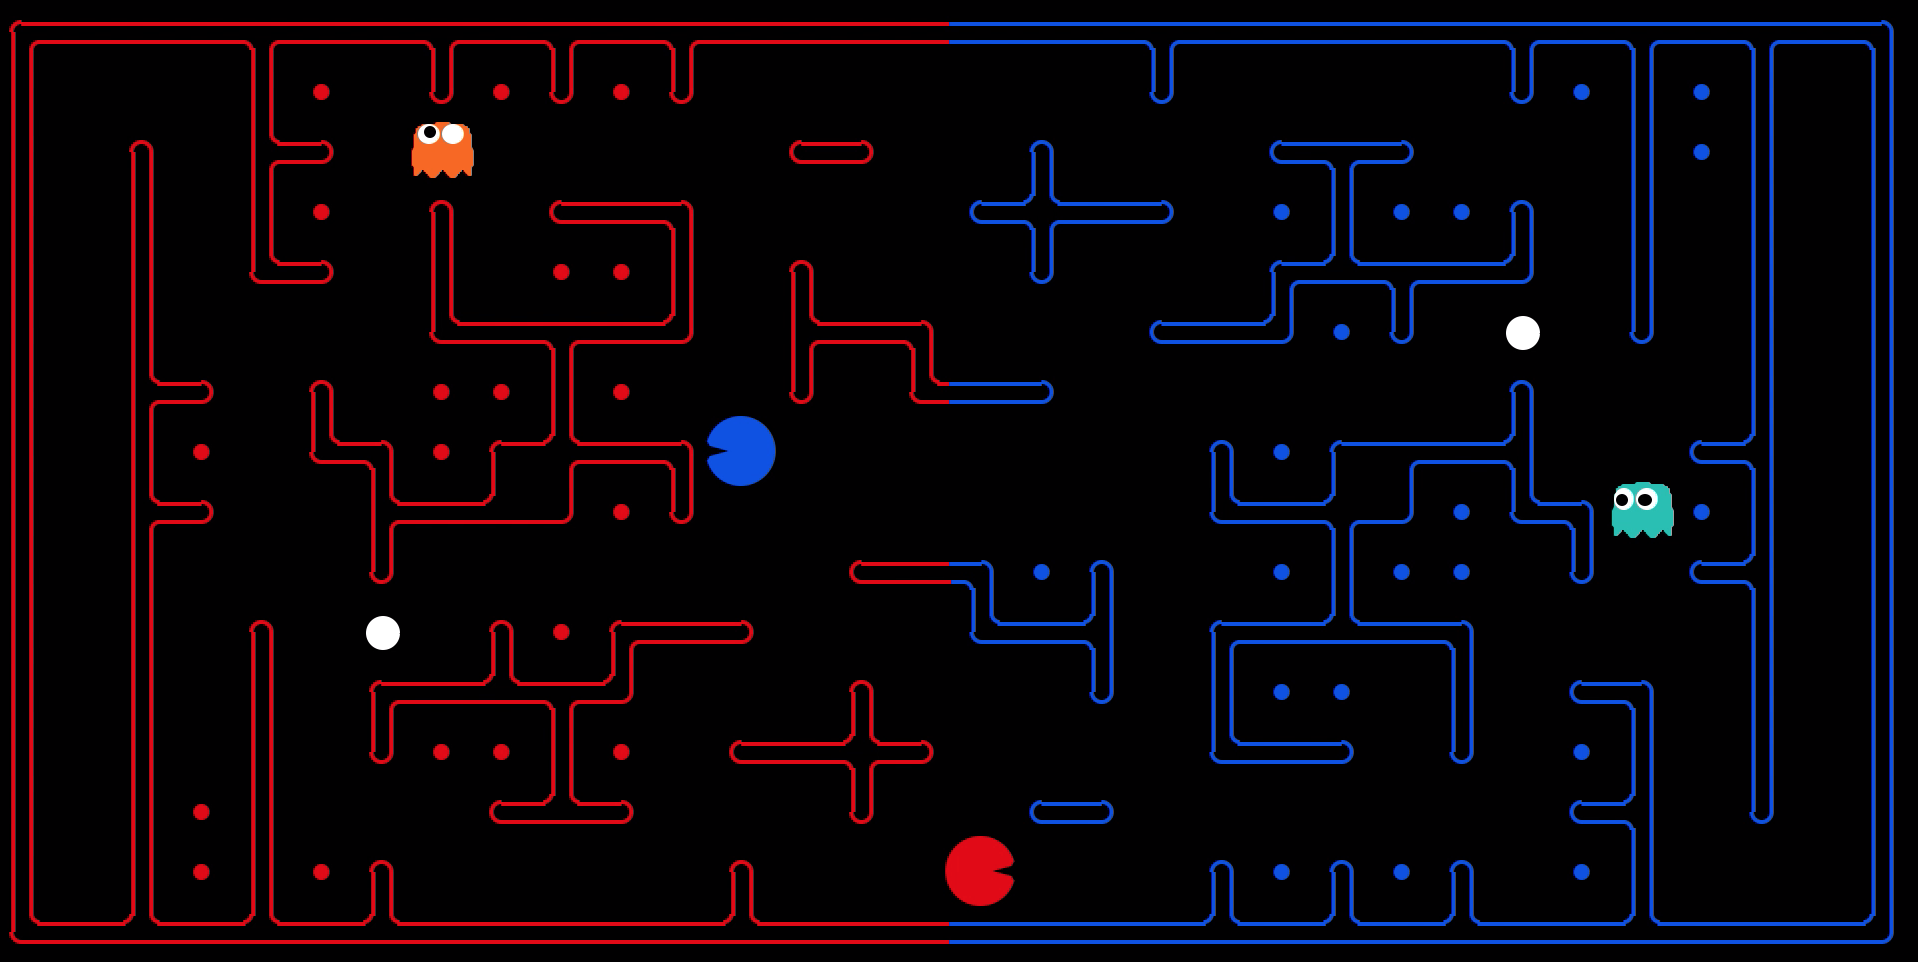
\includegraphics[width=0.5\textwidth]{./figuresA4/pacman_illustration.png}
  \caption{Illustration of environment}
  \label{fig:drag_force}
\end{figure}

% description of figure
The figure shows the game environment, the blue and red dots represent the food pellets, the blue and red lines represent the walls. 
As seen in the figure above there are both Pacman and ghosts. The agent is a ghost when defending its own side. When crossing over to the enemy side to collect pellets it becomes a pacman.
An agent can go into enemy territory and collect pellets, but the score will only increase when the agent returns back to its own side. In the figure there are also white pellets, 
those are power pellets, when an agent collects a power pellet it can eat the enemy agents for a period of 40 moves. During that period the enemy ghost agents are regarded as scared.
When an agent is eaten it respawns at its own side, if the agent was scared before getting eaten it will no longer be scared after respawning.
The game ends when all but two food pellets have been eaten, or when the time limit of 1200 moves has been reached. The team with the highest score wins the game.
There is a limit on calculation time, 15 seconds for initialization and 1 second for each move. If the agent exceeds the time limit three times duting a game the team will forfeit the game.

The information each agent has access to is the following:
\begin{itemize}
  \item The friend agent's positions
  \item The total score
  \item The position of all the food pellets on the map, this is updated every time an agent moves
  \item The position of all the power pellets on the map, this is updated every time an agent moves
  \item The position of an enemy agent if it is within 5 squares of the agent or a teammate
\end{itemize}






\subsection{Task Description}

This report will discuss the problem of developing an agent that can play the game of Pacman capture the flag. 
The aim is to develop two agents which are able to defend their side of the map and also collect food pellets from the enemy side. 
The agents will be able to move in four directions, up, down, left and right. 




These problems and their solutions are addressed in further detail in the following section \ref{rel_work}.




\subsection{Contribution}
% Describe the contribution of the report in detail

In this report we will impement Minimax and alpha-beta pruning into the UC Berkeley Pacman Capture the Flag project. We will also explore the use of Monte Carlo Tree Search (MCTS), Expectimax, and decision-tree-based approaches.
We will also compare the results of our solution with the results of other methods used for the same problem.

An essential aspect of Pacman capture the flag is the ability to cooperate as a team and communicate with the other agent. 
Potential real world applications of this project are many, as the ability of intelligent agents to make strategic decisions in a dynamic environment has many applications. 
Applications include multi-robot system coordination, autonomous vehicles, and unmanned aerial vehicles.







\subsection{Outline}
This report is organized as follows. First we introduce the problem and its importance in section \ref{sec:introduction}. 
Then we discuss and highlight the related work and required backround knowledge in order to understand the proposed solution in section \ref{rel_work}.
This is followed by a detailed description of the proposed solution in section \ref{method}.
Next we present the experimental setup and the results in section \ref{sec:experiments_and_results}.
Finally, we summarize the results and conclude the report in section \ref{sec:conclusion}.












\section{Related Work}
\label{rel_work}
% Describe the related work in detail

The success of AI agents in Pac-Man CTF heavily relies on the choice and implementation of appropriate strategies. This section provides an overview of the relevant research in this domain.

\subsection{Minimax Game Tree Search}
\label{subsec:minimax}
The problem of finding the optimal move in a game can be formulated as a search problem. The search space is a tree, where each node represents a state of the game, and each edge represents a possible move. The root node represents the current state of the game, and the leaf nodes represent the terminal states of the game. The goal is to find the optimal path from the root node to a leaf node. 

The minimax algorithm (shown in Algorithm \ref{alg:minimax}) is a recursive algorithm that computes the optimal move for a player in a two-player game. The algorithm assumes that the opponent plays optimally, and it tries to minimize the maximum loss that can be incurred by the player. It is a classic approach in Game Theory, aiming to find the optimal move in a two-player, zero-sum game. By constructing a game tree and evaluating the utility of different game states, the algorithm enables agents to make informed decisions. 

Sometimes, however, it is not feasible to search the entire game tree, due to the large number of possible moves. To address this issue, the algorithm can be modified to limit the depth of the search tree. The algorithm can also be modified to incorporate heuristics that evaluate the utility of non-terminal game states. Variations of minimax, such as alpha-beta pruning, move ordering based on heuristics, iterative deepening search (IDS), and Repeated States Checking (RSC), have been proposed to improve its efficiency and effectiveness [1][2][3].

\begin{algorithm}
\caption{Minimax Algorithm}
\label{alg:minimax}
\begin{algorithmic}[1]
\Procedure{Minimax}{$node, depth, maximizingPlayer$}
\If{$depth = 0$ or $node$ is a terminal node}
\State \textbf{return} the heuristic value of $node$
\EndIf
\If{$maximizingPlayer$}
\State $value \gets -\infty$
\For{each child of $node$}
\State $value \gets \max(value, \text{Minimax}(child, depth-1, \text{False}))$
\EndFor
\State \textbf{return} $value$
\Else
\State $value \gets \infty$
\For{each child of $node$}
\State $value \gets \min(value, \text{Minimax}(child, depth-1, \text{True}))$
\EndFor
\State \textbf{return} $value$
\EndIf
\EndProcedure
\end{algorithmic}
\end{algorithm}

\subsection{Expectimax}
\label{subsec:expectimax}
Expectimax is a variant of the minimax algorithm that considers uncertain outcomes in games. It is commonly used in domains with probabilistic elements. In Pac-Man CTF, Expectimax can be employed to account for the ghost movement and uncertain states, enabling agents to make rational decisions under uncertainty [6].

\subsection{Monte Carlo Tree Search}
\label{subsec:mcts}
MCTS is a sampling-based search algorithm that has demonstrated remarkable success in various game-playing domains. By combining tree exploration with random rollouts, MCTS performs effective exploration and exploitation of the search space. This approach has been applied to Pac-Man CTF, where agents simulate multiple playouts to estimate the value of different actions and make informed decisions [4][5].


\subsection{Decision Tree Based Approaches}
\label{subsec:decision_tree}
Decision trees offer a structured representation of decision-making processes. By learning from historical data and constructing decision rules, decision-tree-based approaches provide an interpretable framework for agent behavior. These techniques have been explored in Pac-Man CTF, where agents use decision trees to guide their actions based on various game state features [7][8].

\subsection{Hybrid Approaches}
\label{subsec:hybrid}
Several studies have proposed hybrid strategies by combining different AI techniques in Pac-Man CTF. For example, integrating MCTS with minimax or Expectimax algorithms has shown promise in improving agent performance [9][10]. Such hybrid approaches leverage the strengths of different methods to create robust and adaptable AI agents.



\section{Method}
\label{method}
% Proposed method section explaining what you did in more detail

In this section, we will discuss ...





\section{Experiments and Results}
\label{sec:experiments_and_results}

% mention failure to clear intersection with cars
First, we will describe the experimental setup for the two problems, and then we will present the results for each of the problems separately.

\subsection{Experimental Setup}
\label{subsec:experimental_setup}
% Containing the results of other groups in a table, 

\subsubsection{Experimental setup for measurement of performance}
In order to evaluate the performance of the suggested solution, we will compare our approach with five other groups. 
This is done by putting the algorithms against each other in the simulation. 
Two different evaluations will be done, one called pre-finals, in which the groups give their initial solutions, and one called finals, in which after having time to re-evaluate their solutions, the groups give their final solutions.
The results of both evaluations are presented in the tables below.
Results are measured in terms of wins, ties, losses. The score is calculated as the following: 3 points for a win, 1 point for a tie, and 0 points for a loss. The total score is the sum of the points for each group.




\subsection{Results}
\label{subsec:results}
In this section, we summarize the results of our experiments. First we present the results of the two evaluations in the competition, then we present the approach of the winning group.

% table with 5 collumns and 4 rows for the following results:
% 1. Group no. , 2. wins, 3. ties 4. losses 5. total score
% G4, 0, 0, 0, 0
% G2 , 0, 0, 0, 0
% G6 , 0, 0, 0, 0
% G3 , 0, 0, 0, 0
% highlighting G3 

\begin{table}[!hptb]
  \centering
  \begin{tabular}{|c|c|c|c|c|}
    \hline
    \textbf{Group} & \textbf{Wins} & \textbf{Ties} & \textbf{Losses} & \textbf{Total Score} \\
    \hline
    4 & 8 & 0 & 0 & 24 \\
    \hline
    2 & 5 & 1 & 0 & 16 \\
    \hline
    6 & 5 & 1 & 3 & 16 \\
    \hline
    3 & 3 & 5 & 2 & 14 \\
    \hline
  \end{tabular}
  \caption{Results of the pre-finals evaluation.}
  \label{tab:results_prefinals}
\end{table}


% finals results:
% G4: 13 wins, 1 tie, 1 loss, 40 points
% G2: 9 wins, 2 ties, 4 losses, 29 points
% G6: 7 wins, 2 ties, 6 losses, 23 points
% G3: 5 wins, 4 ties, 6 losses, 19 points
\begin{table}[!hptb]
  \centering
  \begin{tabular}{|c|c|c|c|c|}
    \hline
    \textbf{Group} & \textbf{Wins} & \textbf{Ties} & \textbf{Losses} & \textbf{Total Score} \\
    \hline
    4 & 13 & 1 & 1 & 40 \\
    \hline
    2 & 9 & 2 & 4 & 29 \\
    \hline
    6 & 7 & 2 & 6 & 23 \\
    \hline
    3 & 4 & 4 & 6 & 16 \\
    \hline
  \end{tabular}
  \caption{Results of the finals evaluation.}
  \label{tab:results_finals}
\end{table}














\section{Summary and Conclusions}
\label{sec:conclusion}



% \section{Future Work}









% \clearpage
% \newpage
\printbibliography

\newpage

\appendix
% print the appendix title on the top of the page
\section{Appendix}
\label{sec:appendix}








% \paragraph{Relevance of the Problem}
% Collision avoidance is a critical problem in multi-agent systems, where agents must work together to accomplish tasks in a shared environment, where the actions of one agent may affect the state of the environment and the other agents. In this context, collision avoidance is essential to ensure the safety of agents and the success of the mission. This has applications in various domains, including unmanned aerial vehicles, autonomous vehicles, and mobile robots. In these applications, agents must navigate through dynamic and crowded environments while avoiding obstacles and other agents. Thus, developing effective collision avoidance strategies is critical to the reliable and safe operation of multi-agent systems in real-world applications.




% In \cite{6606326}, a novel behaviour tree based control used in decision making processes of robot soccer is proposed.
% The most impressive point is passing.
% The passing behavior tree first controls two robots using parallel sequences, with the passer and receiver aligned, 
% and then the tree checks if the pass is safe. If the ball can be passed, the passer shoots the ball.
% Next, the sequence waits for the ball to start moving, and once this happens, 
% we again wait for the ball to stop, or for the ball to come within the diameter of the receiver's robot, 
% at which point the receiver moves and captures the ball. The use of BT approach allows to model complicated 
% situations easily that show advantages of this technique over finite state machines widely
% used in robot control\cite{6606326}.


% \begin{eqnarray}
%   \label{eqn:car_input}
%   \begin{aligned}
%     % atan(dot product of a and r)
%     \text{steering} &= \arctan(\overrightarrow{\mathbf{a}} \bullet \hat{\mathbf{r}}) \\
%     % atan(dot product of a and f)
%     \text{gas} &= \arctan(\overrightarrow{\mathbf{a}} \bullet \hat{\mathbf{f}}) \\
%     % if magnitude of gas is too small, scale it to 0.2. add a comment about epsilon at the end of the line
%     \text{gas} &= \text{gas} \cdot \frac{\epsilon}{\text{min}(|\text{gas}|, \epsilon)} \\
%     % \text{brake} &= 0 \\
%   \end{aligned}
% \end{eqnarray}

% % figure showing drag
% \begin{figure}[!htbp]
%   \centering
%   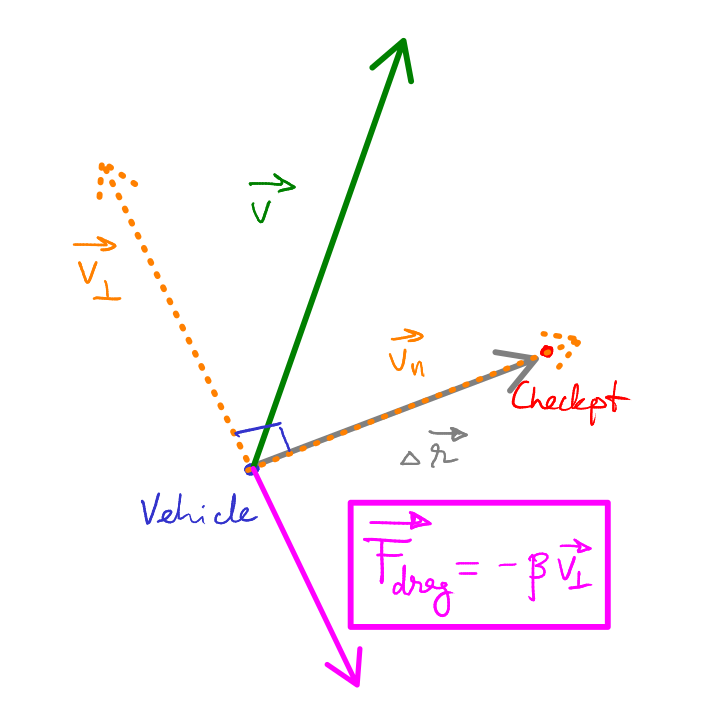
\includegraphics[width=0.3\textwidth]{./figures/intelli_drag.png}
%   \caption{Assistive drag force to help the agent maintain its reference trajectory.}
%   \label{fig:drag_force}
% \end{figure}

% % figure showing velocity obstacle
% \begin{figure}[!hptb]
%   \centering
%   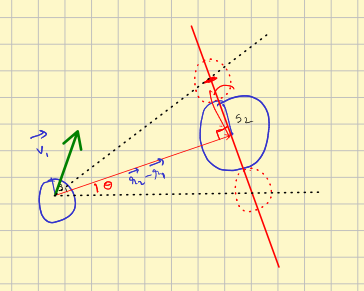
\includegraphics[width=0.3\textwidth]{./figures/VO_repulsion_setup.png}
%   \caption{Velocity Obstacle setup for two agents.}
%   \label{fig:velocity_obstacle_setup}
% \end{figure}


% table layout
% \begin{table}[!hptb]
%   \centering
%   \begin{tabular}{|c|c|c|c|c|c|c|}
%     \hline
%     \textbf{Terrain} & \multicolumn{2}{|c|}{\textbf{Open Field}} & \multicolumn{2}{|c|}{\textbf{Intersection}} & \multicolumn{2}{|c|}{\textbf{Unstructured}} \\
%     \hline
%     \textbf{Group} & \textbf{Circle} & \textbf{Random} & \textbf{Circle} & \textbf{Random} & \textbf{Circle} & \textbf{Random} \\
%     \hline
%     9 & 29 & 28.52 & 44 & 46 & 47 & 40.78 \\
%     \hline
%     13 & 34 & 47 & 55 & 47 & 50 & 47 \\
%     \hline
%     3 & \color{blue}{20.5} & \color{blue}{21} & \color{red}{287} & \color{blue}{32} & \color{blue}{30.5} & \color{blue}{26.5} \\
%     \hline
%     12 & 27.06 & 27.54 & 88.66 & 166.03 & 47.7 & 69.23 \\
%     \hline
%     10 & 42.8 & 42.9 & 64.6 & 158.42 & 52.05 & 69.88 \\
%     \hline
%     16 & 59.4 & 38 & 141.6 & 191.5 & 77.2 & 70.5 \\
%     \hline
%     \textbf{14} & 31.3 & 29.68 & 79.9 & 260.15 & 52.4 & 60 \\
%     \hline
%     \textbf{Overall Best Time} & 20.5 & 21 & 44 & 32 & 30.5 & 26.5 \\
%     \hline
%   \end{tabular}
%   \caption{Completion Times of the top 7 groups with drones on different terrains.}
%   \label{tab:results_drone_CA}
% \end{table}


% % figure showing pseudo traffic lights
% \begin{figure}[!hptb]
%   \centering
%   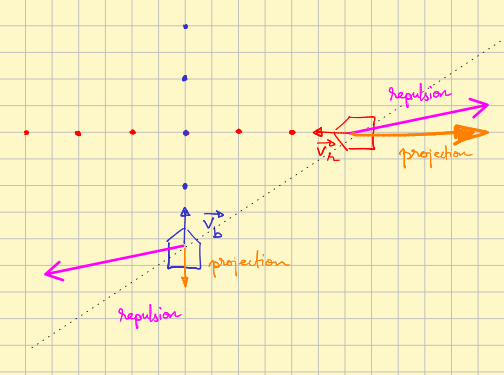
\includegraphics[width= 0.6\textwidth]{./figures/pseudo_traffic_lights.png}
%   \caption{Pseudo-traffic lights. Note that the repulsion force is only along the direction of the path. So the red car slows down a lot, while the blue car does not decelerate as much. The blue car can pass the intersection before the red car, without steering away from its original path.}
%   \label{fig:pseudo_traffic_lights}
% \end{figure}


% % figure showing ball chasing
% \begin{figure}[!hptb]
%   \centering
%   \begin{subfigure}[b]{0.45\textwidth}
%     \centering
%     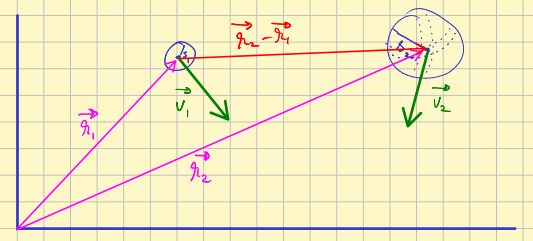
\includegraphics[width=\textwidth]{./figures/soccer_VO_attraction_setup.png}
%     \caption{VO\_Attraction Setting}
%     \label{fig:soccer_VO_attraction_setting}
%   \end{subfigure}
%   ~
%   \begin{subfigure}[b]{0.45\textwidth}
%     \centering
%     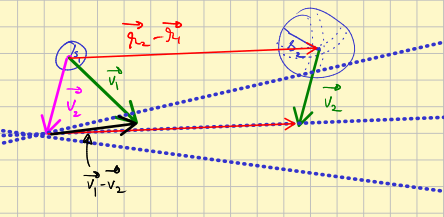
\includegraphics[width=\textwidth]{./figures/soccer_VO_attraction_setup_2.png}
%     \caption{VO\_Attraction Initial Setup}
%     \label{fig:soccer_VO_attraction_initial_setup}
%   \end{subfigure}
%   \caption{Setup for our Ball-chasing strategy.}
% \end{figure}



% table comparing results of different groups (drones)

% \begin{table}[!hptb]
%   \centering
%   \begin{tabular}{|c|c|c|c|c|c|c|}
%     \hline
%     \textbf{Terrain} & \multicolumn{2}{|c|}{\textbf{Open Field}} & \multicolumn{2}{|c|}{\textbf{Intersection}} & \multicolumn{2}{|c|}{\textbf{Unstructured}} \\
%     \hline
%     \textbf{Group} & \textbf{Circle} & \textbf{Random} & \textbf{Circle} & \textbf{Random} & \textbf{Circle} & \textbf{Random} \\
%     \hline
%     9 & 29 & 28.52 & 44 & 46 & 47 & 40.78 \\
%     \hline
%     13 & 34 & 47 & 55 & 47 & 50 & 47 \\
%     \hline
%     3 & \color{blue}{20.5} & \color{blue}{21} & \color{red}{287} & \color{blue}{32} & \color{blue}{30.5} & \color{blue}{26.5} \\
%     \hline
%     12 & 27.06 & 27.54 & 88.66 & 166.03 & 47.7 & 69.23 \\
%     \hline
%     10 & 42.8 & 42.9 & 64.6 & 158.42 & 52.05 & 69.88 \\
%     \hline
%     16 & 59.4 & 38 & 141.6 & 191.5 & 77.2 & 70.5 \\
%     \hline
%     \textbf{14} & 31.3 & 29.68 & 79.9 & 260.15 & 52.4 & 60 \\
%     \hline
%     \textbf{Overall Best Time} & 20.5 & 21 & 44 & 32 & 30.5 & 26.5 \\
%     \hline
%   \end{tabular}
%   \caption{Completion Times of the top 7 groups with drones on different terrains.}
%   \label{tab:results_drone_CA}
% \end{table}




\end{document}
